\chapter{Prestazioni}
Analizziamo ora le prestazioni degli algoritmi presentati nei capitoli  \textit{\ref{chap.BitonicSort}} e \textit{\ref{chap.QuickSort}}. I risultati che verranno presentati sono stati raccolti eseguendo, per ogni variazione dei parametri, un numero di test variabile tra 2 e 6. Come input sono stati utilizzati 7 diversi file di input generati casualmente che contengono numeri interi nell'intervallo $[0,999]$. La taglia massima dell'input è stata scelta a causa di una limitazione imposta dall'utilizzo della libreria OpenMPI sul calcolatore IBM Power7 utilizzato per i test. Utilizzando questa libreria, infatti, non è possibile allocare più di 120MB di memoria. Dovendo memorizzare due copie dell'array di input (una per ogni algoritmo), avendo alcune allocazioni aggiuntive e dovendoci limitare ad utilizzare un numero di elementi pari ad una potenza di 2 la taglia massima è stata scelta come 8'388'608 elementi (circa 32MB).

\begin{figure}[H]
\centering
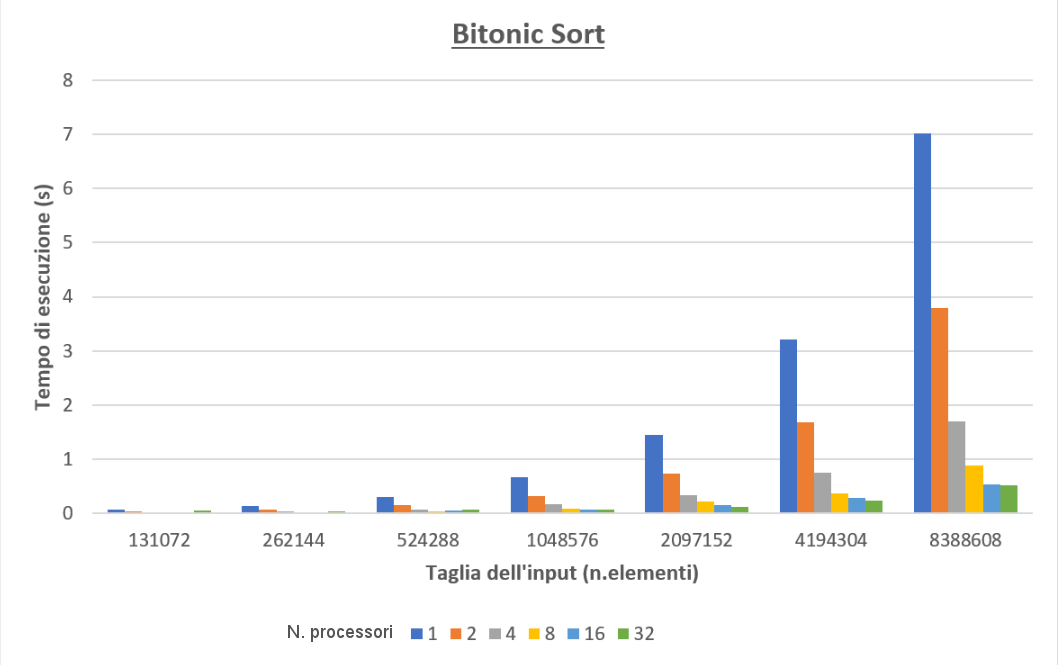
\includegraphics[scale=0.35]{images/BitonicSort}
\caption{\footnotesize{Tempo di esecuzione di Bitonic Sort al variare di input e numero di processori utilizzati.}}\label{img.BitonicSort}
\end{figure}

Nella \textit{Figura \ref{img.BitonicSort}} si possono vedere i tempi di esecuzione di Bitonic Sort al variare della taglia dell'input (da 131'072 elementi fino a 8'388'608 elementi) e al variare del numero di processori utilizzati. Si può notare come fino a 16 processori i tempi scalino molto bene, mentre nel passaggio tra 16 e 32 processori il miglioramento è ridotto. L'aumento della taglia dell'input comporta un aumento significativo nei tempi di esecuzione.
Possiamo analizzare lo speedup più in dettaglio nella \textit{Figura \ref{img.SpeedupBitonic}}, che rappresenta i tempi di esecuzione con un input di 8'388'608 elementi. Come si poteva intuire del grafico precedenze, fino a 8 processori il tempo praticamente dimezza. Nel passaggio a 16 e 32 processori l'overhead aumenta, ma abbiamo comunque un aumento di prestazioni. Probabilmente, se venissero eseguiti test con un numero maggiore di processori, l'overhead diventerebbe eccessivo.
\begin{figure}
\centering
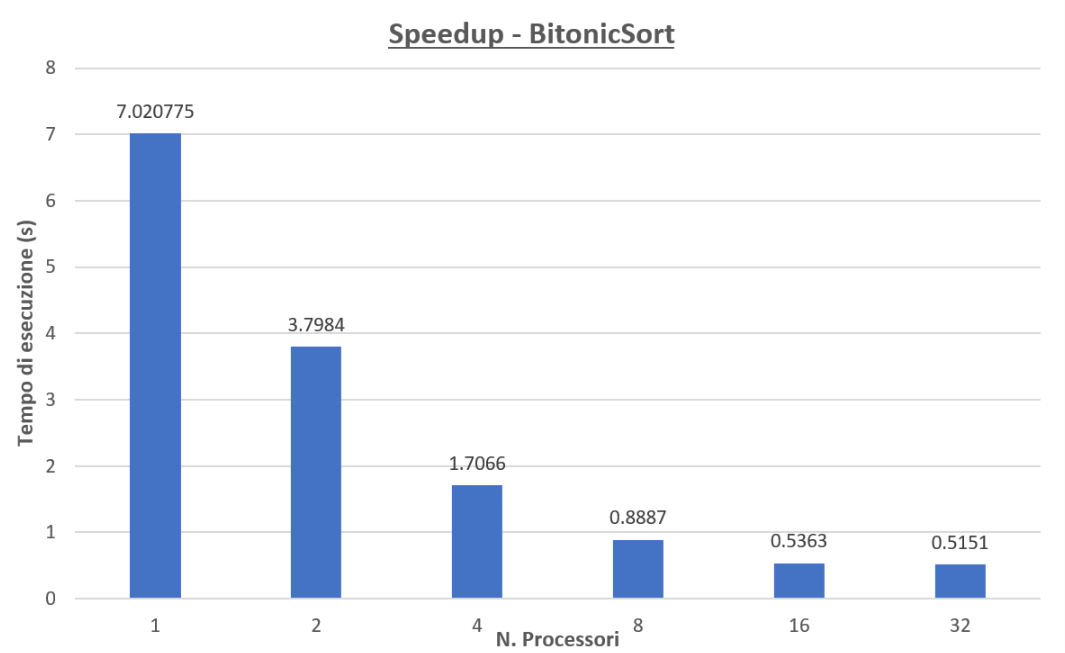
\includegraphics[scale=0.35]{images/SpeedupBitonic}
\caption{\footnotesize{Speedup di Bitonic Sort al variare del numero di processori utilizzati.}}\label{img.SpeedupBitonic}
\end{figure}

Vediamo ora gli stessi grafici per quanto riguarda Quick Sort.
\begin{figure}
\centering
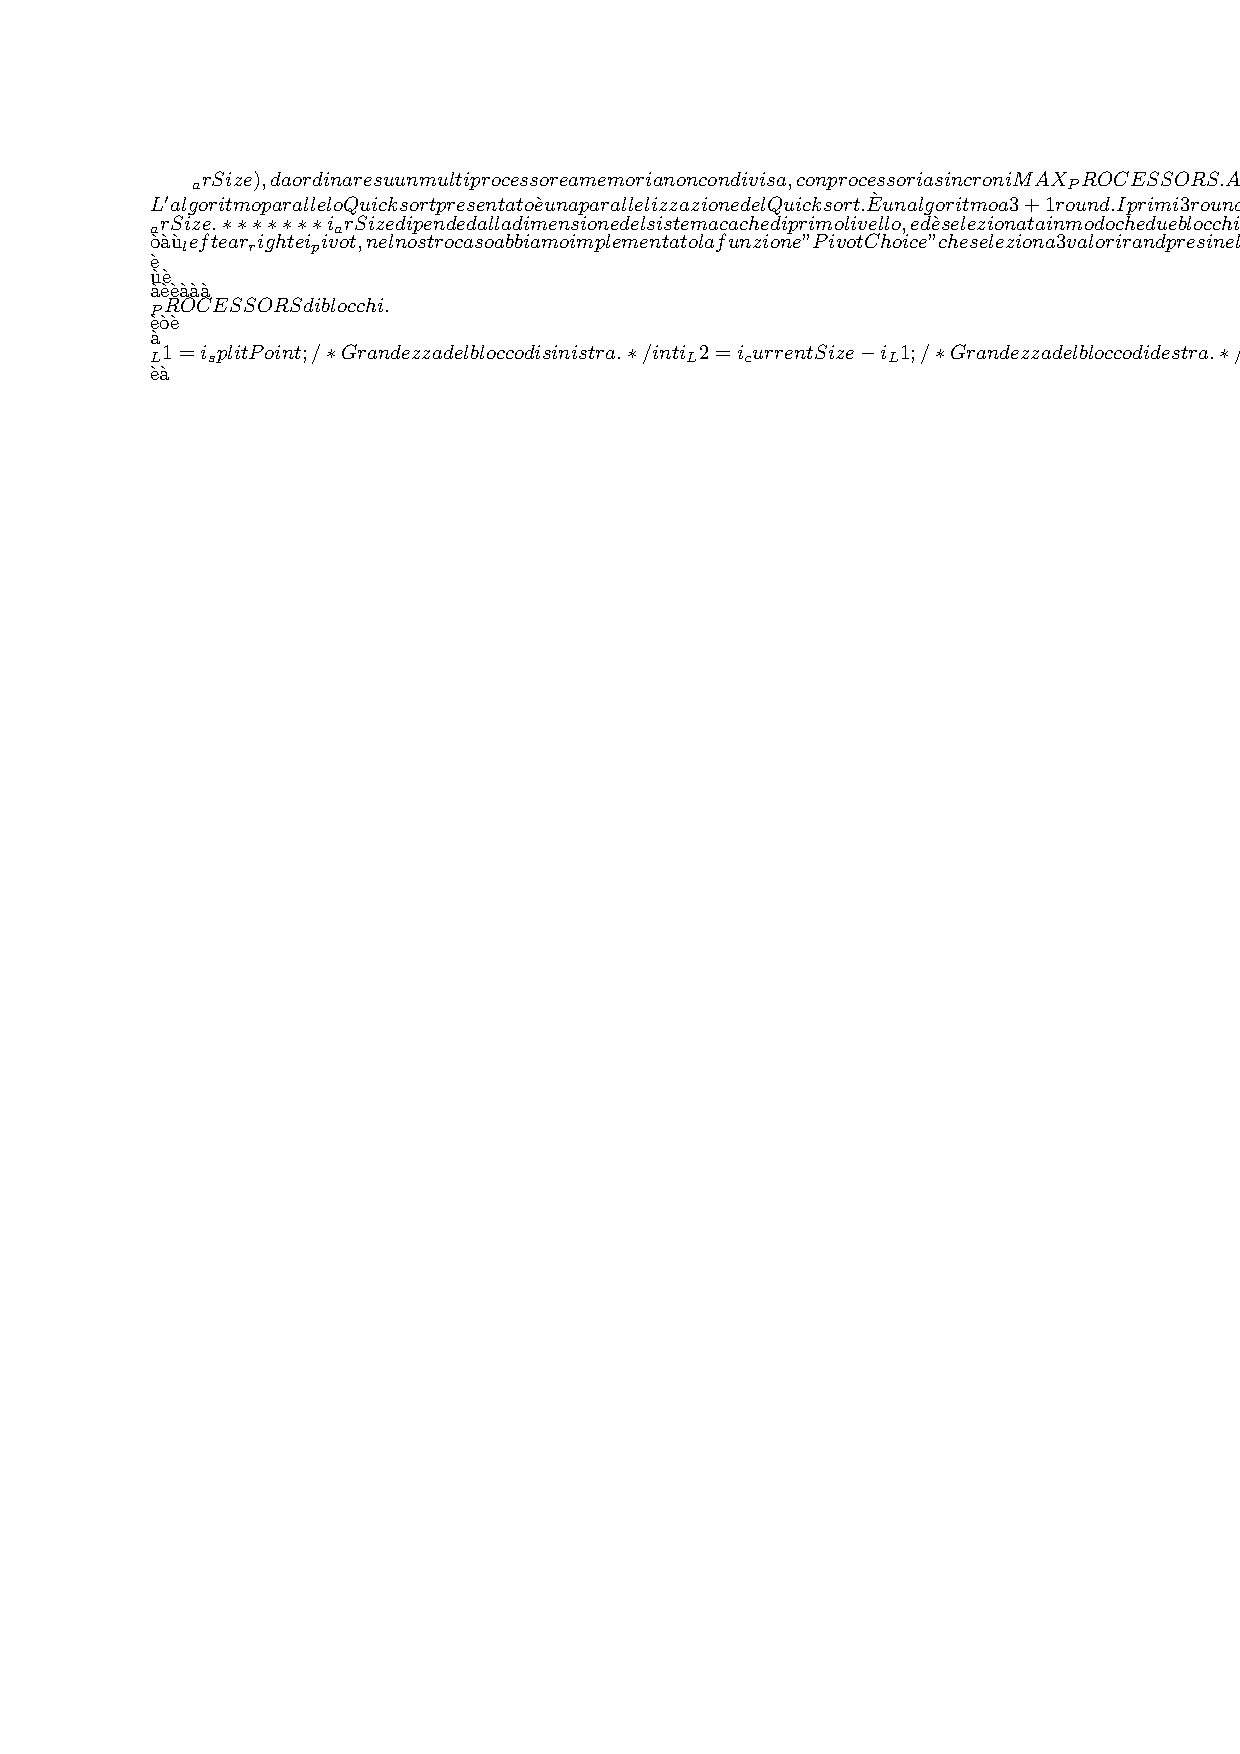
\includegraphics[scale=0.35]{images/QuickSort}
\caption{\footnotesize{Tempo di esecuzione di Quick Sort al variare di input e numero di processori utilizzati.}}\label{img.QuickSort}
\end{figure}
\begin{figure}
\centering
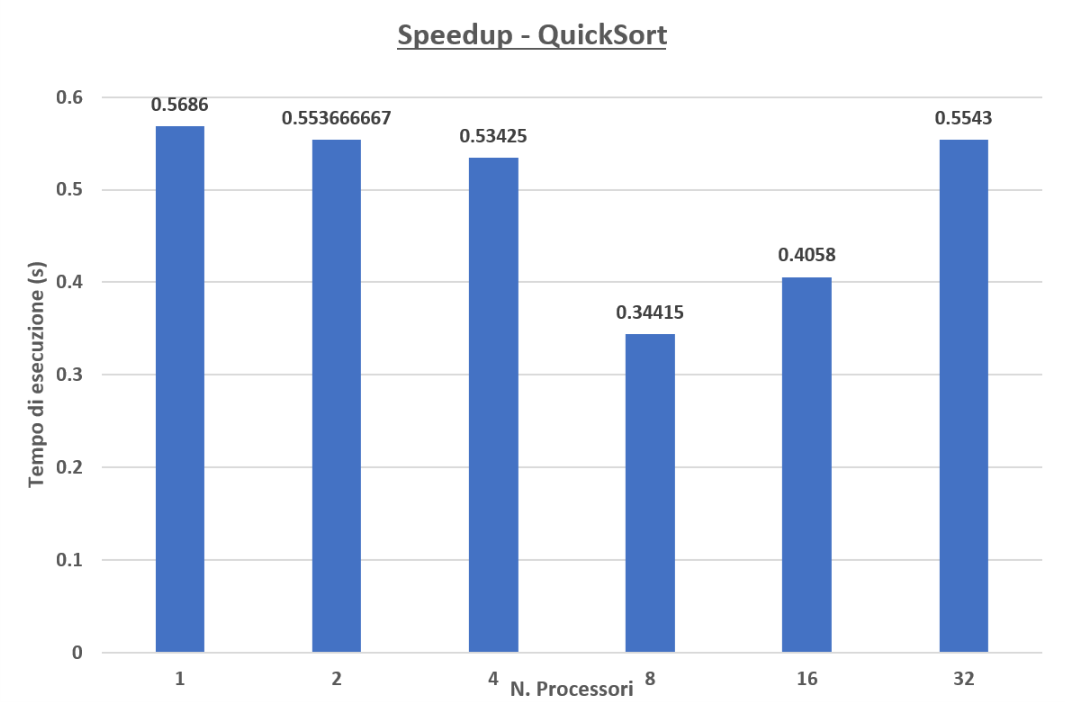
\includegraphics[scale=0.35]{images/SpeedupQuick}
\caption{\footnotesize{Speedup di Quick Sort al variare del numero di processori utilizzati.}}\label{img.SpeedupQuick}
\end{figure}
Possiamo subito vedere come i tempi di esecuzione, pur essendo generalmente più rapidi di quelli di Bitonic Sort, non scalano in modo eccessivo con il numero di processori. In particolare possiamo osservare come, fino a 4 processori, i miglioramenti siano quasi impercettibili. Il passaggio a 8 processori, che risulta essere il valore ottimale, comporta una riduzione dei tempi di circa il 40\%. Aumentando ulteriormente il numero di processori, l'overhead delle numerose sincronizzazioni effettuate risulta troppo oneroso rispetto al vantaggio di suddividere il carico tra più processori.

\begin{figure}
\centering
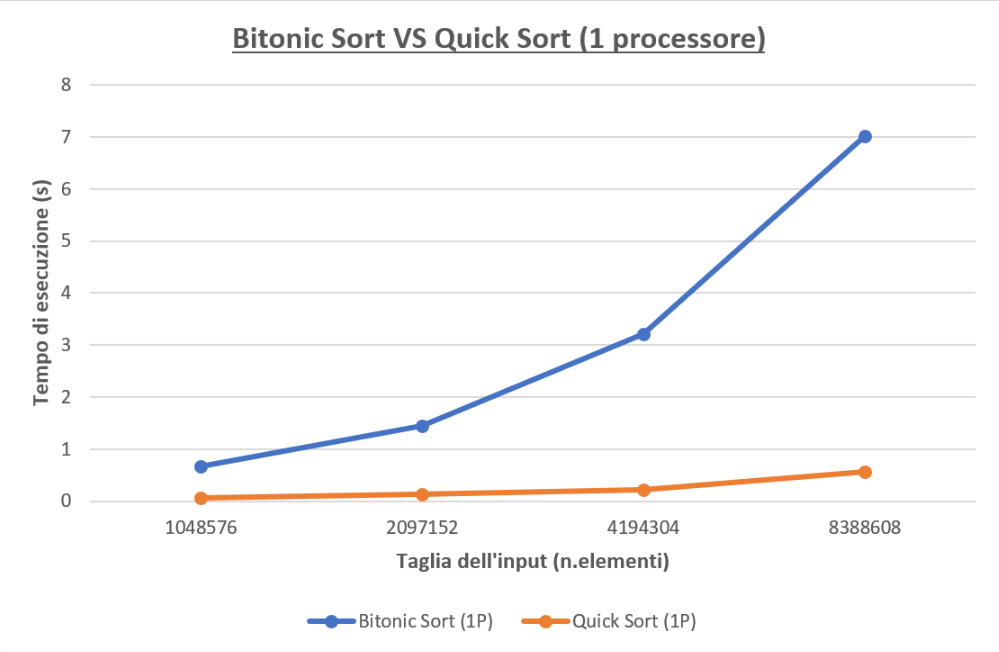
\includegraphics[scale=0.3]{images/BitonicVSQuick1P}
\caption{\footnotesize{Tempi di esecuzione di Bitonic Sort e Quick Sort al variare dell'input utilizzando 1 processore.}}\label{img.BitonicVSQuick1P}
\end{figure}

Andiamo ora a confrontare i risultati dei due algoritmi, in modo da stabilire in quali casi si possa preferire uno rispetto all'altro.
Per prima cosa osserviamo le prestazioni dei due algoritmi utilizzando un singolo processore (\textit{Figura \ref{img.BitonicVSQuick1P}}). In questo caso in cui entrambi gli algoritmi eseguono un ordinamento sequenziale, saltando le parti di comunicazione proprie di un'esecuzione parallela, possiamo vedere come QuickSort risulti più veloce per qualunque taglia di dell'input.
Andiamo a vedere ora le analisi nei casi ottimi dei due algoritmi (8 processori per Quick Sort e 32 per Bitonic Sort, \textit{Figura \ref{img.BitonicVSQuick8-32P}}). 

\begin{figure}
\centering
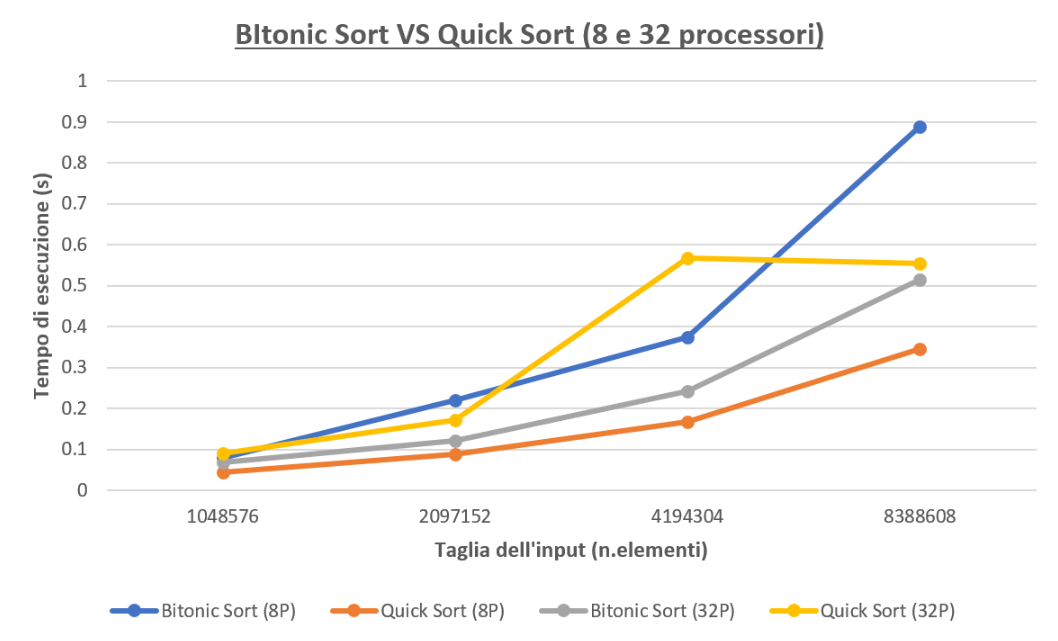
\includegraphics[scale=0.3]{images/BitonicVSQuick8-32P}
\caption{\footnotesize{Tempi di esecuzione di Bitonic Sort e Quick Sort al variare dell'input utilizzando 8 e 32 processori.}}\label{img.BitonicVSQuick8-32P}
\end{figure}

Si nota immediatamente come per input piccoli i due algoritmi (utilizzati con il loro numero ottimale di processori) siano abbastanza ravvicinati, mentre all'aumentare del numero di elementi Quick Sort con 8 processori risulti più rapido di Bitonic Sort con 32. Le prestazioni di Bitonic Sort con 8 processori sono comprensibilmente inferiori rispetto a quelle con 32 processori. Quick Sort, d'altra parte, quando eseguito con 32 processori fornisce risultati erratici. Per stabilirne il comportamento in modo accurato servirebbe un numero maggiore di test eseguiti su una maggior varietà di input.
C'è da notare, inoltre, che le esecuzioni di Quick Sort con 16 e 32 processori risentono di un bug, non ancora identificato, che porta due elementi fuori posto e rende l'output dell'algoritmo non ordinato. In teoria questo non dovrebbe alterare le prestazioni dell'algoritmo in modo significativo, ma per esserne sicuri bisognerebbe dedicare tempo aggiuntivo per risolvere il problema.